\section{Symmetry Breaking In 8-Connected Grid Maps}
\label{cha::rsr::symm8c}
We now describe a variation of the rectangle-based symmetry breaking technique
from Section~\ref{cha::rsr::symm4c} which is applicable to 8-connected grid
maps.  The generalisation is more challenging than it might look at a first
glance.  On a 4-connected map no perimeter node requires more than one
macro-edge (to the closest node on the opposite side of the perimeter) to
retain optimality.  Thus, it is easy to maintain a low branching factor.  In
the 8-connected case many more macro edges are needed to preserve optimality.

A straightforward generalisation approach would be to add a macro-edge between
any two nodes on the perimeter of a rectangle.  We will call the sub-graph
resulting from such an operation a \emph{perimeter clique}.  Although the
perimeter clique approach guarantees optimality, it has the disadvantage of
creating a large branching factor and slowing down search (the number of
necessary macro edges for a rectangle is quadratic in the number of perimeter
nodes).  We will therefore introduce an alternative strategy, that creates
fewer macro-edges, by defining a \emph{dominance} relation between
macro-edges.

\begin{definition}
\label{def:dominance}
A macro-edge connecting two arbitrary nodes $t_1$ and $t_2$ in a perimeter
clique is non-dominated if all other paths between $t_1$ and $t_2$ in the
perimeter clique have a cost strictly larger than the macro-edge at hand.
\end{definition}

By starting with a perimeter clique and applying Definition
\ref{def:dominance} it is easy to see that the set of non-dominated
macro-edges are precisely the ones that we identify below.  There are three
cases to discuss: connections between nodes on the same rectangle side,
connections between orthogonal rectangle sides, and connections between
opposite rectangle sides.  In the discussion that follows note that the cost
of each added macro-edge is equal to the heuristic distance between its two
endpoints -- as measured using $h_{OD}$ or octile distance 
(we describe this heuristic in Chapter~\ref{cha::lit::heuristics}).

The first case is simple: adjacent nodes on the same perimeter side are connected
just as in the original grid. 
In the second case, two nodes on orthogonal sides of the perimeter of a rectangle
$R$ are connected \emph{iff} the shortest path between them is a diagonal
(45-degree) line; this is illustrated in Figure \ref{fig::rsr::macroedges} (left).
Notice that in both cases we introduce no more than two macro edges per node.
In the third case, we generate for each perimeter node a ``fan'' of neighbours
from the opposite side $R$.  Figure \ref{fig::rsr::macroedges} (right), illustrates
this idea.  Starting from a node such as $t_{1}$ we step to the closest
neighbour from the opposite side of $R$ and extend the fan by progressing away
from the middle in both directions adding each node we encounter.  The last node
on either side of the fan is placed diagonally, at 45 degrees, from $t_{1}$
(such as $t_{2}$) or located in the corner of the perimeter (whichever we
encounter first).  There is no need to add further nodes, such as $t_{3}$, as
these can be reached optimally from $t_1$ via the path $\lbrace t_1, t_2, \dots,
t_3\rbrace$.

\begin{figure}[tb]
       \begin{center}
		   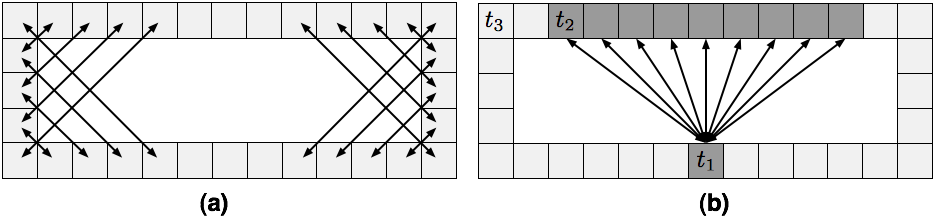
\includegraphics[width=0.95\columnwidth, trim = 10mm 10mm 10mm 0mm]
			{chapter_rsr/diagrams/macroedges_wide.png}
       \end{center}
	\vspace{-3pt}
       \caption[Rectangular Symmetry Reduction on 8-connected maps]
{\small
(Left) Macro edges between nodes on orthogonal sides of an empty
rectangle. (Right) Each node on the perimeter is connected to a set of 
nodes on the opposite side.}
       \label{fig::rsr::macroedges}
\end{figure}

In the rest of this chapter we will use macro-edge to refer to a non-dominated
macro-edge.  We show next that the non-dominated macro-edges computed using
our strategy are both necessary and sufficient to ensure optimal traversal
between any two perimeter nodes.

\begin{proposition} All non-dominated macro-edges are necessary to ensure
optimal paths in a perimeter clique.  
\end{proposition} 
\begin{proof} By
definition, a non-dominated macro-edge $e$ is the only way to travel optimally
between its end nodes in a perimeter clique. Therefore, dropping $e$ would
result in losing path optimality in the perimeter clique.  
\end{proof}

\begin{lemma} \label{lemma::rsr::rooms} Let $R$ be an empty rectangle in
an 8-connected grid map. Let $m$ and $n$ be two perimeter locations.
Then, $m$ and $n$ can be connected optimally through a path that
contains only non-dominated macro-edges.
\end{lemma}

\begin{proof}
We split the proof over the 3 cases discussed earlier: 1) {$m$ and $n$ are on
the same side of the perimeter;} 2) {\label{lemma::rsr::rooms-step2}$m$ and
$n$ are on orthogonal sides of the perimeter;} and 3)
{\label{lemma::rsr::rooms-step3} $m$ and $n$ are on opposite sides of the
perimeter.}

In the first case we can simply walk along the perimeter from $m$ to $n$; the
optimality of this path is immediate. In the second and third case we argue as
follows: the two nodes can be connected through an optimal path that has one
diagonal macro-edge (either at the beginning of the path or at the end) and
zero or more straight macro-edges.  See again the example of travelling from
$t_1$ to $t_3$ in Figure
\ref{fig::rsr::macroedges} (Right).
\end{proof}

\noindent
\textbf{Node Insertion:}
Sometimes a node from the interior of an empty rectangle is required as a start
or goal location for an agent.  To handle such situations we give an online
procedure that temporarily re-inserts nodes back into the map for the duration
of a search.  It proceeds as follows: {If the start and goal are interior nodes
in the same room no insertion is necessary; an optimal path is trivially
available. } {On the other hand, if the start and goal are not in the same
rectangle, add four ``fans'' (collections) of macro edges.  Each fan connects
the start (goal) node to a set of nodes on one side of the rectangle's
perimeter.  Fans are built as shown earlier.}

Given the simple geometry of rectangles, it is possible to identify in constant
time the set of nodes which the start or goal must be connected to.  Further,
these neighbours could be generated on the fly.

\begin{lemma}
\label{lemma::rsr::insertion}
Let $R$ be an empty rectangle in an 8-connected grid map.  For any
nodes $m$, $n$, with $m$ a re-inserted interior node and $n$ a node on the
perimeter, it is always possible to find an optimal cost path which mentions
no interior nodes except for $m$.
\end{lemma}
\begin{proof}
Our re-insertion procedure connects the start or goal to a set of nodes on each
side of $R$.  The procedure in each case is the same as the one given when
connecting two nodes on opposite sides of $R$.  To prove optimality we can
simply run the argument given for Step 3 of Lemma \ref{lemma::rsr::rooms} for each
node on the perimeter of $R$, in each case substituting $m$ for the newly
inserted node.
\end{proof}

We claim that eliminating symmetries as outlined earlier
preserves the completeness and the solution optimality:
\begin{theorem}
For every optimal path $\pi$ on an original grid, there exists an optimal path
$\pi'$ on the modified graph with the property that $\pi$ and $\pi'$ have the
same cost.
\end{theorem}
\begin{proof}
Consider an optimal path $\pi$ on the original map and a rectangle $R$ that is
crossed by $\pi$.  Let $m$ and $n$ be the two perimeter points along $\pi$.
According to Lemma~\ref{lemma::rsr::rooms}, there is a way to connect $m$ and $n$
optimally in the modified graph. Thus, we can replace the original segment $[m
\dots n]$ in $\pi$ with the cost-wise equivalent segment that corresponds to the
modified graph.  The case when $m$ (or $n$) is the start or goal node is
addressed similarly using Lemma~\ref{lemma::rsr::insertion}.  By performing such a
path segment replacement for all rectangles intersected by $\pi$, we obtain a
path $\pi'$ that satisfies the desired properties.
\end{proof}

